\chapter{Project Management}\label{chapter 7}

\section{Methodology}
The methodology of this project can be divided into two parts, Research Methodology and Test Methodology.\\

\textbf{Research Methodology:}\\
This project originally aimed to study the community detection problem with the help of group theory. This choice was motivated by two factors: firstly, group theory is a powerful tool for analysing structural properties, making it a natural extension to graph theory; secondly, I am more familiar with abstract algebra. However, there are very few papers in this field, and most of them either focus on very small graphs or Cayley graphs, which are graphs constructed from groups. Both of these approaches do not fit this project very well. As a result, I had to shift my focus to the mainstream research in the field of community detection. After extensive research, I realised that there are numerous variants of the community detection problem, each with different graph models, benchmarks, and consequently, different types of approaches. My supervisor and I decided to focus on community detection under the stochastic block model (SBM) because it proposes a phase transition phenomenon. However, as discussed in the previous chapter, the easy regime (SNR > 1) has been solved. Therefore, we had to focus our attention on the hard regime, but its hardness is supported by Theorem \ref{thm:1.1.2}. Hence, we needed some extra information, and the reasoning for the choice of extra information is discussed in Chapter \ref{chapter:3}. Since we only have a local information, and one suitable algorithm dealing with local information is the greedy algorithm, if our approach is local optimal, then we have the hope that it might not be very distant from the globally optimal solution. The reasoning for the details of greedy algorithm is discussed in section \ref{sec: greedy recovery}.\\

\textbf{Test Methodology:}\\
The evaluation of the greedy recovery algorithm is based on the following functions:
\begin{itemize}
    \item \textit{generate\_SBM(n, c\_in, c\_out, communities\_size):}  This function generates a graph with 2 built-in communities, where the inner-cluster probability is $c_{in}/n$ and the across-cluster probability is $c_{out}/n$. It also returns the true community assignment $\sigma$.
    \item \textit{generate\_SBM\_improved(n, c\_in, c\_out, communities\_size):} This function generates a graph with multiple communities and the true assignment $\sigma$. To speed up the \textit{generate\_SBM} function when generating a graph with multiple communities, I utilise the function \textit{nx.stochastic\_block\_model(sizes, p, nodelist=None, seed=None, directed=False, selfloops=False, sparse=True)} from \url{https://networkx.org/documentation/stable/reference/generated/networkx.generators.community.stochastic_block_model.html}
\end{itemize}
The evaluation of the spectral algorithm is based on the following function:
\begin{itemize}
    \item \textit{non\_backtracking\_matrix(G):} This function constructs a non-backtracking matrix based on the graph $G$.
\end{itemize}
All implementations of the above functions are listed in the Appendices.

\section{Software Used}
\begin{itemize}
    \item \textbf{Jupyter Notebook:} All implementations in this project are coded using Jupyter Notebook.
    \item \textbf{Overleaf:} This report is written in \LaTeX~on Overleaf.
    \item \textbf{GitHub:} GitHub is used for version control of both the implementations and the final report.
    \item \textbf{Chatgpt:} Chatgpt is used for proofreading and polishing some pieces of the final report.
\end{itemize}

\section{Time Management}
\begin{figure}[ht]
    \centering
    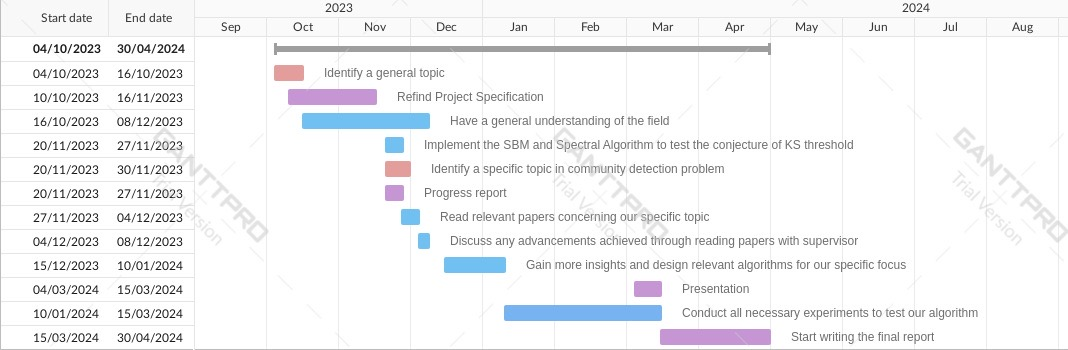
\includegraphics[width=1\linewidth]{Figures/Project Timeline.jpeg}
    \caption{Project Timeline}
    \label{fig:enter-label}
\end{figure}
Term 1 was primarily dedicated to reading papers to gain an overview of the subject. However, I fell slightly behind schedule during this term due to two main reasons. Firstly, papers in this area generally required more time to digest than I had anticipated. Secondly, I was exploring potential topics, such as clustering with noisy queries, graph clustering via min-cut, and community detection via group action, in order to identify a specific topic that I could pursue.\\
Once the specific topic was determined, tasks in Term 2 proceeded smoothly. I completed all tasks on time and had extra time to explore some other interesting directions that were still within the scope of this project, such as the combined algorithm.
